\par
At the quarterly scale, the proportionality gap can be examined over a fixed three-quarter horizon. In the full distributed-lag specification, the contemporaneous elasticity is $c_0=\DynamicNow$ [\DynamicNowLow, \DynamicNowHigh] and the complete response through the third subsequent quarter is $c_3=\DynamicEnd$ [\DynamicEndLow, \DynamicEndHigh]. The two-sided test of $c_3=1$ gives $p=\DynamicEndP$. A stipulated persistent 10\% facility difference corresponds to \DynamicNowTen\% [\DynamicNowTenLow, \DynamicNowTenHigh] higher conditional weekly activity initially and \DynamicEndTen\% [\DynamicEndTenLow, \DynamicEndTenHigh] by the endpoint; the latter interval remains below the proportional 10\% benchmark. Table~\ref{tab:quarterly_dynamic} gives the static, one-lag and three-lag estimates, while Figure~\ref{fig:dynamic} displays the endpoint path and the covariance-based lag contrast.

The additional follow-through is the covariance-based contrast $c_3-c_0=\DynamicExtra$ [\DynamicExtraLow, \DynamicExtraHigh], with $p=\DynamicExtraP$. Its interval includes both negative and positive increments. Thus the endpoint response supports a finite-horizon subproportional relationship, while the contrast does not isolate a delayed increment beyond the contemporaneous association. The $c_L$ endpoint and the $c_3-c_0$ contrast answer different questions and use the full clustered covariance; neither is cumulative activity nor evidence of later parity. Complete coefficient terms, finite-lag paths and the pandemic-index comparison are reported in SI Section~\siref{sec:si-quarterly}; the intermediate $h=2$ interval includes unit elasticity.

The main support contains \DynamicRows{} rows in \DynamicCities{} cities from \DynamicStart{} to \DynamicEndQuarter, including \DynamicPositiveRows{} positive and \DynamicZeroRows{} source-coded-zero outcomes. The retained quarters have complete compatible-week coverage, $W/W^{\mathrm{cal}}=1$, as an observed support property. Static and one-quarter specifications use exactly the same observations as the three-lag model: their estimates are \StaticQuarter{} [\StaticQuarterLow, \StaticQuarterHigh] and \OneLagQuarter{} [\OneLagQuarterLow, \OneLagQuarterHigh], respectively.

The pandemic-context comparison uses \CovidDynamicRows{} rows in \CovidDynamicCities{} cities and \CovidDynamicProvinces{} province clusters. Its terminal elasticity is \CovidBase{} [\CovidBaseLow, \CovidBaseHigh] without the response index and \CovidAdjusted{} [\CovidAdjustedLow, \CovidAdjustedHigh] with the index. This paired result describes how the conditioning variable changes the estimate within the available subset; it does not assign the difference from the full-period estimate to pandemic exposure.
\begin{table}[htbp]\centering\small\caption{Quarterly facility--activity estimates}\label{tab:quarterly_dynamic}
\begin{tabular}{@{}p{52mm}rrr@{}}\toprule
Quantity & Static & One lag & Three lags\\
\midrule
$c_0$ [95\% CI] & 0.739 [0.498, 0.980] & 0.659 [0.356, 0.962] & 0.682 [0.408, 0.955]\\
$c_L$ [95\% CI] & 0.739 [0.498, 0.980] & 0.736 [0.495, 0.976] & 0.737 [0.497, 0.977]\\
$c_L-c_0$ [95\% CI] & -- & 0.077 [-0.119, 0.273] & 0.055 [-0.097, 0.208]\\
$p(c_L=1)$ & 0.034 & 0.032 & 0.032\\
$p(c_L-c_0=0)$ & -- & 0.440 & 0.474\\
Conditional activity difference for a 10\% facility increase (\%) [95\% CI] & 7.29 [4.86, 9.79] & 7.27 [4.83, 9.75] & 7.28 [4.85, 9.76]\\
City--quarters / cities & 1,542 / 111 & 1,542 / 111 & 1,542 / 111\\
\bottomrule\end{tabular}\end{table}

\begin{figure}[htbp]\centering
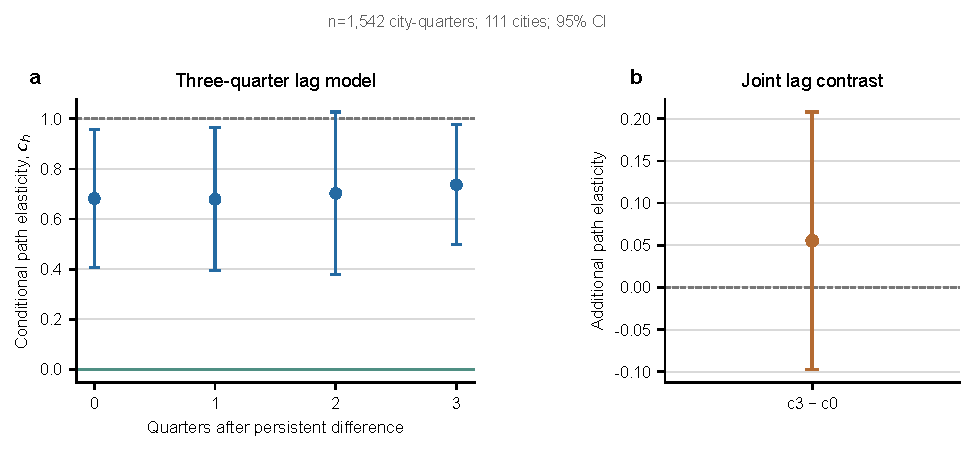
\includegraphics[width=\linewidth]{figures/fig7_quarterly_dynamic.pdf}
\caption{Quarterly facility--activity relationships}\label{fig:dynamic}
\end{figure}

\FloatBarrier
